\chapter{Sistema de telecomunicaciones}\label{comunicacion}
Se determinó utilizar la plataforma Arduino por su simplicidad en prototipado y programación, además de ser de fácil acceso y una tecnología escalable. En base a esto se decide comenzar a trabajar en el apartado de comunicación.
\section{Redes móviles, Bluetooth y Android}
Como se comentó anteriormente, la primera elección de tecnología para la comunicación fue la de utilizar redes móviles directamente, esto por medio del módulo GPRS Shield. Este es un módulo de comunicación 2G compatible con socket XBee para la Arduino UNO (un socket XBee dota a una placa Arduino de la capacidad de comunicarse en forma inalámbrica \cite{xbee_info}). Para comodidad se escogió una variante de Arduino UNO llamado PICARO+, la cual posee entre otras modificaciones el socket XBee integrado.\\
Para esta comunicación se debe hacer uso tanto de la placa principal, el chip de comunicación y una antena, estas últimas 2 mencionadas en las figuras \ref{gprs} y \ref{antena}.\\
Dentro de las características del GPRS se encuentran el emplear una tarjeta SIM, conector SMA y el chip Quectel M95. En cuanto a la antena nos encontramos con cuatri-banda: 
\begin{enumerate}
	\item\textbf{GSM/850E: 824 a 894 [MHz]}
	\item\textbf{GSM: 880 a 960 [MHz]}
	\item\textbf{DCS: 1710 a 1880 [MHz]}
	\item\textbf{PCS: 1850 a 1990 [MHz]}
\end{enumerate}

\newpage
Si bien puede parecer cuestionable el utilizar tecnología 2G, es importante considerar que chip provee de hasta 85.6 [kbps] y diversos protocolos de comunicación. Con lo cual al año 2017 (se espera deshabilitar las redes 2G en el mediano plazo para dar paso a nuevas tecnologías) sirve como prueba de concepto dado su bajo costo y el acercamiento que ofrece a los comandos AT, los cuales son los empleados para controlar chips de este tipo.
Luego de comenzado el proceso de configuración, se encontraron diversos problemas con esta elección:

\begin{enumerate}
	\item\textbf{Dimensiones:}
	Dado que este módulo esta contemplado para operar en conjunto con la placa principal, se hace engorroso el tener una antena de casi 6 [cm] y de gran grosor adosado al cuerpo del paciente.
	\item\textbf{Consumo energético:}
	Este módulo hace necesario el uso de una fuente de alimentación externa de mayor capacidad (9[V] aproximadamente) respecto a la necesidad base de la placa (3.3[V]), lo que conlleva a usar un cargador externo y en su momento a una batería de mayor capacidad.
	\item\textbf{Antigüedad de comandos:}
	Los comandos Hayes (también llamados AT \cite{AT}) son un conjunto de comandos empleados en la configuración y parametrización de módems, su uso data de al menos 1990 y en cierto punto dejaron de usarse para dar paso a controladores específicos. 
	\item\textbf{Tasas de transferencias:}
	A raíz de un estudio preliminar en tasas de transferencia se estableció que alrededor de 150 datos por segundo debían ser enviados (esto en función de las tasas de operación de un ECG común\cite{ecg_rate}), por tanto el usar esta tecnología obliga a emplear 3G como mínimo. 
	\item\textbf{Costo:}
	En comparación a otras tecnologías indirectas de redes móviles como lo puede ser el Bluetooth, la inversión necesaria es mayor y su flexibilidad bastante menor.
\end{enumerate}

Por todo lo anterior, se pasa a una segunda iteración en busca de emplear tecnología Bluetooth y un intermediario para llegar a las redes celulares.\\


\section{Perfiles Bluetooth}

Bluetooth \cite{bluetooth} es una especificación industrial para Redes Inalámbricas de Área Personal (WPAN) creado por Bluetooth Special Interest Group, Inc. que posibilita la transmisión de voz y datos entre diferentes dispositivos mediante un enlace por radiofrecuencia en la banda ISM de los 2.4 GHz y data de 1994 y actualmente se encuentra en su versión 5.0. La versión a emplear en este proyecto es la 4.0 llamada BLE (Bluetooth Low Energy) que se detalla en capítulos adelante. \\

Un perfil Bluetooth es la especificación de una interfaz de alto nivel para su uso entre dispositivos Bluetooth. Para utilizar Bluetooth, un dispositivo debe implementar alguno de los perfiles soportados.
Los perfiles son descripciones de comportamientos generales que los dispositivos pueden utilizar para comunicarse, formalizados para favorecer un uso unificado. La forma de utilizar las capacidades de Bluetooth se basa, por tanto, en los perfiles que soporta cada dispositivo. Los perfiles permiten la manufactura de dispositivos que se adapten a sus necesidades.\\

A la fecha existen más de 27 perfiles Bluetooth, pero durante el desarrollo del proyecto se emplearon solo dos: SPP y GATT, los cuales se detallarán en su momento.

Las principales diferencias entre estos últimos dos perfiles son: GATT pertenece al estándar introducido en la versión 4.0 (desde ahora BLE) mientras que SPP en la versión 2.1. BLE está pensado para operar con un consumo energético inferior que versiones anteriores, posee mayor velocidad en el establecimiento de la conexión y está pensado para la transferencia de pequeñas cantidades de datos. Excepto por el último punto se puede observar una notoria superioridad de GATT (BLE) frente a SPP, pero como se verá más adelante, las tasas de transferencias obtenidas con GATT son lo suficientemente buenas como para escogerla en este proyecto.

\newpage
\section{Razones para Android}

Para seleccionar el intermediario entre la comunicación Bluetooth y las redes móviles se decidió un teléfono inteligente, por sus capacidades de cómputo, gran accesibilidad y flexibilidad al ofrecer un entorno de desarrollo propio de su sistema operativo. Ahora bien, para seleccionar el sistema operativo se recurre a su penetración en el mercado y como se puede observar en la figura \ref{market_share} Android se alza como el gigante en el mercado.

\begin{figure}[H]
	\centering
	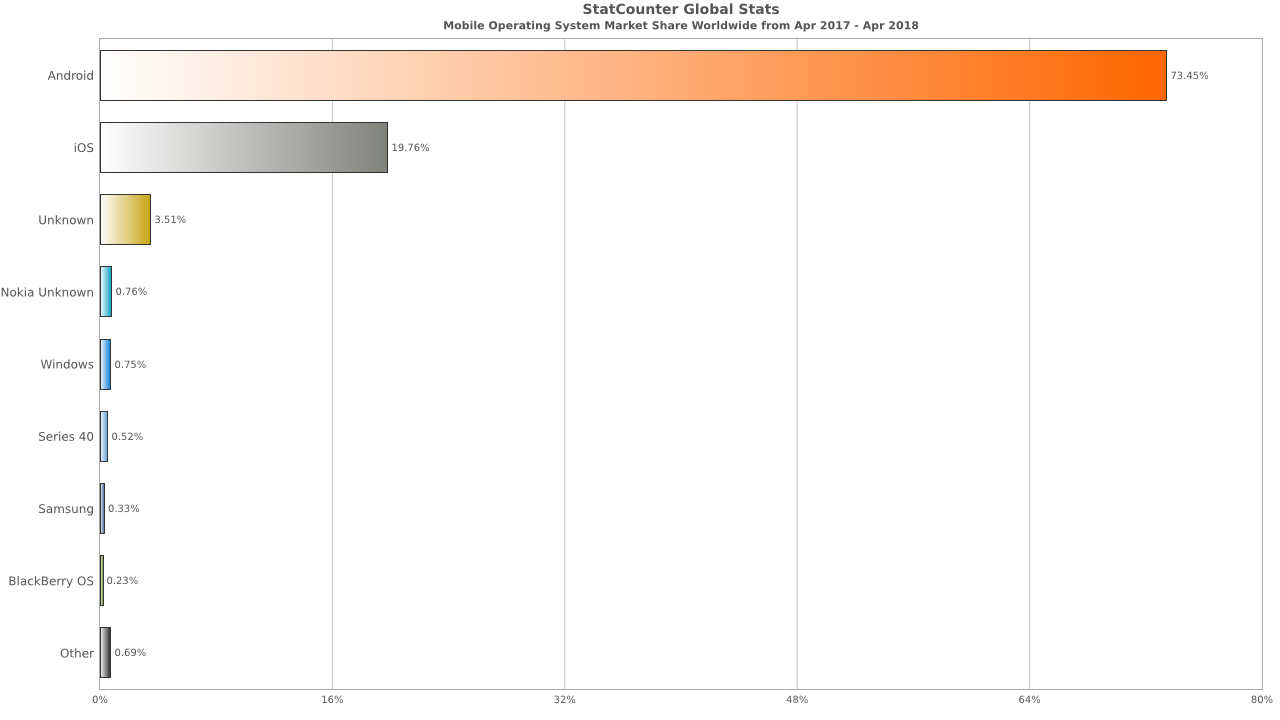
\includegraphics[scale=0.4]{figuras/comunicacion/Market_share.png}
	\caption{Mercado compartido mundial de sistemas operativos móviles 2017-2018 \cite{market_share_cita}}
	\label{market_share}
\end{figure}

Además de lo anterior, se ha de considerar el entorno de desarrollo y el ecosistema que rodea al sistema operativo en cuestión. En el caso de Android, se trabaja principalmente con Android Studio (Para sistemas Linux, Windows y Mac), en lenguaje Java o Kotlin, con una comunidad activa de desarrolladores y una gran cantidad de librerías a disposición.\\
Por último se considera la accesibilidad de los terminales, con lo cual es de conocimiento general que Apple posee precios más elevados que los dispositivos Android.
Por lo tanto se concluye que Android es la mejor alternativa en estos momentos.

\newpage
\section{Comparativa desarrollo híbrido}
Para el desarrollo móvil actual existen dos grandes aproximaciones, las cuales pasan principalmente por el uso de entornos de desarrollo que permiten el despliegue en más de un sistema operativo (llamados híbridos) o uno determinado con un solo código fuente.\\

Primero, en el ámbito nativo (un código fuente para un despliegue único): 

\begin{table}[H]
	\centering
	\begin{tabular}{| c | c | c | c |}
		\hline
		\multicolumn{1}{|c|}{\textbf{OS}}&
		\multicolumn{1}{c|}{\textbf{Lenguaje}}&
		\multicolumn{1}{|c|}{\textbf{IDE}}&
		\multicolumn{1}{|c|}{\textbf{Plataforma}}\\ \hline
		Android  & Java, Kotlin  & Android Studio, Eclipse & Linux, Mac, Windows \\ \hline
		iOS  & Objective-C, Swift & XCode & Mac \\ \hline
	\end{tabular}
	\caption{Comparativa de desarrollo nativo, elaboración propia}
	\label{native_comparative}
\end{table}

Continuando con el ámbito híbrido, se destacan 3 grandes competidores:

\begin{table}[H]
	\centering
	\begin{tabular}{| c | c | c |}
		\hline
		\multicolumn{1}{|c|}{\textbf{Framework}}&
		\multicolumn{1}{c|}{\textbf{Tipo de resultado}}&
		\multicolumn{1}{|c|}{\textbf{Lenguaje}}\\ \hline
		Ionic  & No nativo  & JavaScript (AngularJS) \\ \hline
		Reac Native  & Nativo & JavaScript (React) \\ \hline
		Flutter  & Nativo & Dart \\ \hline
	\end{tabular}
	\caption{Comparativa de desarrollo híbrido, elaboración propia}
	\label{hybrid_comparative}
\end{table}

Por último se analizan ventajas y desventajas de ambas aproximaciones al desarrollo móvil, cabe destacar que Flutter aún en 2018 se encuentra en fase beta, pero se considera por las grandes prestaciones que presenta (por lo que no se considerarán sus ventajas en la siguiente tabla), además se establece un marco en donde se espera obtener un desarrollo tanto para iOS como para Android:

\begin{table}[H]
	\centering
	\begin{tabular}{| c | c | c |}
		\hline
		\multicolumn{1}{|c|}{\textbf{Característica}}&
		\multicolumn{1}{c|}{\textbf{Nativo}}&
		\multicolumn{1}{|c|}{\textbf{Híbrido}}\\ \hline
		Rendimiento  & Máximo  & Suficiente \\ \hline
		Actualizaciones SO  & Sin retraso & Con retraso \\ \hline
		Librerías  & Extenso & Acotado \\ \hline
		Control  & Total & Parcial \\ \hline
		Tiempo de desarrollo  & Alto & Medio/bajo \\ \hline
		Cantidad de código  & Alto & Mínimo \\ \hline
		Diversidad de código  & Total & Unificado \\ \hline
		Complejidad  & Alta & Baja \\ \hline
	\end{tabular}
	\caption{Desarrollo nativo versus híbrido, elaboración propia}
	\label{native_hybrid}
\end{table}

Como se puede observar en la tabla \ref{native_hybrid}, el mayor potencial para el desarrollo híbrido es cuando no se tienen funcionalidades demasiado específicas (que requieran librerías especiales), no se requiere gran rendimiento, no se utilizarán las últimas características de seguridad del SO y el tiempo es primordial.\\
Si bien se podría considerar el uso híbrido, se espera que la aplicación haga uso de alto poder de procesamiento, utilice librerías específicas (como graficar en tiempo real como se verá más adelante) y se tenga el mayor control posible de todos los procesos. Por lo tanto se descarta el uso de entornos híbridos para el desarrollo, en desmedro de la compatibilidad con dispositivos Apple.


\newpage
\section{Prueba de concepto}

Para comenzar el desarrollo e iniciar los sucesivos Sprint (metodología SCRUM), se hizo uso del perfil SPP de Bluetooth, incluído en su versión 2.1 + EDR (2004) y que permite comunicación bidireccional. Es uno de los perfiles fundamentales de Bluetooth al tener un comportamiento muy parecido a los de la comunicación serial (como la usada en conexiones RS-232 o UART).
Está basado en el protocolo RFCOMM y emula una linea serial, para su uso se utilizan dos actores, uno que actúa como servidor y otro que actúa como cliente. El primero queda a la espera de alguna conexión entrante (visible), luego por medio de una búsqueda y el uso de un UUID el segundo genera una conexión para comenzar a intercambiar datos.

El objetivo es generar una prueba de concepto por el cual se usara a una aplicación Android como puente para llevar información internet.

Para esto se implementó la siguiente arquitectura:

\begin{figure}[H]
	\centering
	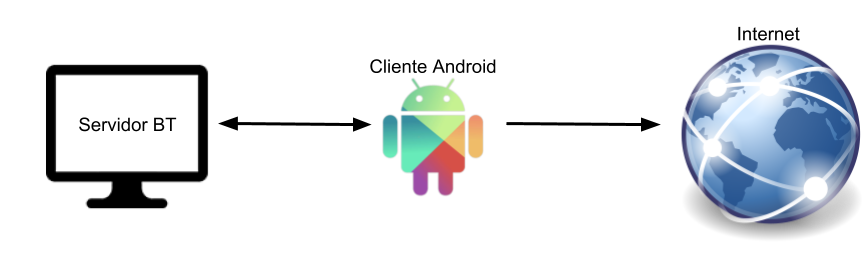
\includegraphics[scale=0.4]{figuras/comunicacion/prueba.png}
	\caption{Arquitectura de la prueba de concepto. Fuente: Elaboración propia}
	\label{prueba_concept}
\end{figure}

Como se puede observar en la figura \ref{prueba_concept} el servidor Bluetooth ()desarrollado en Java) fue implementado en computador (Windows), mientras que la aplicación Android básica permite el escaneo, selección y conexión con el servidor Bluetooth. Esto último sin utilizar librerías externas.

La prueba resultó exitosa, pudiendo enviar información (cadenas de texto) desde el computador hasta una página web previamente configurada, la cual se detallará en el siguiente capítulo. Cabe destacar que el uso de este perfil Bluetooth fue solo por simplicidad y próximamente se hará uso de un perfil acorde al proyecto.